\documentclass[10pt,conference]{IEEEtran}
% DRAFT v1 (2026-11-15) of the IJCNN 2027 revision.
% Sections I-VI are written; method details reflect the locked protocol v2.
% Everything inside \pending{...} waits for the main study and must not be
% read as a result. Remove the \pending macro's colour before submission.

\usepackage{amsmath,amssymb,amsfonts}
\usepackage{booktabs}
\usepackage{graphicx}
\usepackage{cite}
\usepackage{xcolor}
\usepackage[hidelinks]{hyperref}

\graphicspath{{figures/}}

\newcommand{\PH}{ProtoHedge}
\newcommand{\DeepH}{Deep Hedging}
\newcommand{\pending}[1]{\textcolor{red}{[PENDING: #1]}}

\begin{document}

\title{ProtoHedge on Historical Option Data: A Controlled Comparison with Deep Hedging and Delta-Based Hedges}

\author{\IEEEauthorblockN{Anonymous Authors}}

\maketitle

\begin{abstract}
ProtoHedge, introduced by Faloughi, Guo and Luk, makes a learned hedging
policy inspectable by expressing each trade as a weighted average of actions
attached to real past market states, and was reported to match Deep Hedging
in simulated markets. We reproduce that result with the authors' code and
then test the method on 34,395 historical option episodes from ten U.S.
underlyings, against Deep Hedging and two textbook hedges, with the same
inputs, objective and tuning budget for both learned families. With the
original settings neither family learns to hedge on historical data. With a
hedging-error objective and outputs defined as corrections to the delta
hedge, both beat the delta hedge in all ten underlyings out of sample. Deep
Hedging reduces the standard deviation of the hedging error to 0.40
(European call) and 0.61 (Asian call) of the delta hedge's; ProtoHedge
reaches 0.69 and 0.81, is behind Deep Hedging in every underlying, and is
behind a delta--vega hedge in most. Training one ProtoHedge model on all ten
underlyings removes most of this deficit. Three prototypes reproduce a
ProtoHedge decision closely, but with the released encoder the heaviest
prototype is the most similar past state in only 28\% of decisions; a
plain-distance layer raises this to 76\% and hedges better.
\end{abstract}

\begin{IEEEkeywords}
deep hedging, interpretable machine learning, prototype networks, option
hedging, risk-sensitive learning
\end{IEEEkeywords}

\section{Introduction}

A trader who has sold an option must trade other instruments over the option's
life so that gains on those trades offset the payment owed at expiry. This is
hedging: a sequential decision problem with transaction costs, position limits
and an uncertain terminal loss. The classical answer is the delta hedge, which
holds the underlying asset in proportion to the option's price sensitivity
\cite{black1973pricing}. \DeepH{} (DH) replaces the formula with a neural
network trained end to end on a risk measure of the terminal outcome
\cite{buehler2019deep}. It can account for costs and several hedging
instruments, but an individual trade is hard to explain.

\PH{} (PH), introduced by Faloughi, Guo and Luk
\cite{faloughi2025protohedge}, is an interpretable alternative. It is not our
method; this paper evaluates it. PH keeps DH's objective and replaces the
network's output by a weighted average of actions attached to a small library
of \emph{prototypes}, each a market state that actually occurred in the
training data. A decision can then be read as ``the current state resembles
these past states, which carry these actions''. The original study reported
that PH matches DH to within 0.4\% of utility in two simulated markets, and
listed historical data and path-dependent options as open questions.

We take up those questions. On simulated paths a method can be trained on
thousands of independent samples from a known process. Historical option data
are different in ways that matter for learning: a ticker offers roughly a
hundred non-overlapping monthly paths, prices drift, contracts expire, and
neighbouring episodes overlap. A fair historical test must therefore answer
three questions in order.
\begin{enumerate}
\item Does each learned policy hedge at all, measured against textbook hedges
on the dispersion of the hedging error and not only on the training utility?
\item When DH and PH receive the same data, inputs, objective and tuning
budget, how close does PH come to DH?
\item Do the prototype explanations of real trades say what they appear to
say?
\end{enumerate}

Our contributions are as follows.
\begin{itemize}
\item \emph{Reproduction.} With the original authors' code we reproduce the
simulated near-parity of PH and DH, and document that PH fails to train in a
minority of restarts, which the single runs of the original study could not
show (Section~\ref{sec:repro}).
\item \emph{A controlled historical protocol.} Ten U.S. underlyings, two
liabilities, fixed listed contracts, chronological splits, identical inputs
and equal tuning budgets for both model families, two textbook hedges as
references, and inference that respects dependence across time and across
assets (Sections~\ref{sec:setup}--\ref{sec:eval}).
\item \emph{What makes learning work.} With the original objective and trade
outputs, neither family learns to hedge on historical data: both end with
four to six times the delta hedge's dispersion. Training on the variance of
the hedging error, with the output defined as a correction to the delta
hedge, makes both families train in every one of 300 fits
(Section~\ref{sec:ablation}).
\item \emph{Three-way results.} Out of sample, both families beat the delta
hedge in all ten underlyings. DH also matches or beats a delta--vega hedge.
PH is behind DH in every underlying, by a factor of 1.3 to 1.7 in the
standard deviation of the hedging error (Section~\ref{sec:main}). The deficit
shrinks as training data grow, and one PH model trained on all ten
underlyings recovers most of it.
\item \emph{An audit of the explanations.} With ten prototypes, three of them
carry 92\% of a decision's weight and reproduce it closely. Whether the
heaviest prototype is a similar market state depends on the layer: 28\% of
decisions with the released encoder, 76\% with the plain layer
(Section~\ref{sec:explain}).
\end{itemize}

\section{Background and Related Work}

\subsection{Deep Hedging}
Let $x_t$ be the information available at decision time $t$. DH trains a
network $\pi_\theta$ that maps $x_t$ to a trade, by minimising a risk measure
of the terminal outcome over whole episodes \cite{buehler2019deep}. Variants
use reinforcement learning \cite{kolm2019dynamic,cao2021deep} or value-based
formulations such as QLBS \cite{halperin2020qlbs}; risk-averse policy search
traces a frontier between cost and risk \cite{vittori2020option}. The output
parameterisation matters for trainability: a network that outputs a
no-transaction band trains faster and more reliably than one that outputs
trades \cite{imaki2021notransaction}.

\subsection{ProtoHedge}
PH \cite{faloughi2025protohedge} builds on prototype networks, which classify
by similarity to learned or selected examples
\cite{li2018prototypes,chen2019looks} and are interpretable by construction
rather than after the fact \cite{rudin2019stop}. PH has three steps.
\begin{enumerate}
\item \emph{Collect states.} Train a DH agent and record every state it visits
on the training episodes.
\item \emph{Select prototypes.} Standardise the states, cluster them with
$K$-means \cite{macqueen1967}, and keep the real visited state nearest to
each centre. The $K$ prototypes $p_1,\dots,p_K$ are fixed from here on.
\item \emph{Learn actions.} Attach a trainable bounded action $b_k$ to each
prototype and train, with DH's objective, the policy
\begin{equation}
 \alpha_{t,k}=\frac{\exp(-d(x_t,p_k))}{\sum_j \exp(-d(x_t,p_j))},\qquad
 \pi(x_t)=\sum_{k=1}^{K}\alpha_{t,k}\,b_k .
 \label{eq:proto}
\end{equation}
\end{enumerate}
The weights $\alpha_{t,k}$ and actions $b_k$ are the computation itself, so
the decomposition of a decision is exact. What ``similar'' means depends on
the distance $d$. In the released code, states and prototypes pass through a
small trainable encoder $f_\phi$ and
$d(x,p)=\lVert f_\phi(x)-f_\phi(p)\rVert^2$ (the \emph{encoder} layer). An
earlier layer, which the authors' notebooks show was used for their
Black--Scholes result, measures distance in the input space,
$d(x,p)=\sum_j w_j (x_j-p_j)^2$ (the \emph{plain} layer). We evaluate both,
because only the plain layer guarantees that a heavily weighted prototype is
a nearby market state.

\subsection{Learned hedging on historical option data}
Deep reinforcement-learning hedgers have been trained on intraday S\&P~500
option prices \cite{mikkila2023empirical}. On S\&P~500 and Euro Stoxx~50
options a hedging network reduces the squared hedging error relative to the
Black--Scholes hedge, but a linear regression that captures the leverage
effect does about as well \cite{ruf2022hedging}; simple references are
therefore essential. A recent study finds that reinforcement-learning hedgers
on S\&P~500 options learn a small correction to the delta hedge whose benefit
is fragile across regimes, and distils the policy into formulas
\cite{zernikov2026deep}. Risk measures that are only weakly risk-averse let a
learned hedger profit from drift in the training data instead of hedging
\cite{buehler2021drift}. To our knowledge no study has evaluated a
prototype-based hedging policy on historical option data.

\section{Problem Setup}
\label{sec:setup}

\subsection{The hedging task}
Each episode has $T=20$ daily decisions. At the start the hedger is short one
synthetic call option on the underlying, struck at the initial price $S_0$.
For the \emph{European} call the payment at the end is $\max(S_T-S_0,0)$; for
the arithmetic-average \emph{Asian} call \cite{kemna1990asian} the terminal
price is replaced by the mean of the 20 daily closing prices after the start.
The hedger may trade two instruments each day: the underlying and one listed
call option on it. All prices are divided by $S_0$.

Let $P_t\in\mathbb R^2$ be the two instrument prices, $h_t$ the positions held
after trading at $t$, $a_t=h_t-h_{t-1}$ the trade, $\kappa_t$ the cost per
unit traded, and $H\le 0$ the payment owed. The premium-excluded outcome is
\begin{equation}
 O=H+\sum_{t=0}^{T-1}h_t^\top(P_{t+1}-P_t)-\sum_{t=0}^{T-1}\kappa_t^\top|a_t| ,
 \label{eq:offset}
\end{equation}
and the \emph{hedging error} is $E=O+V_0$, where $V_0$ is a model value of the
liability at the start (Black--Scholes for the European call, a
moment-matching approximation for the Asian call, both with the listed call's
implied volatility). $V_0$ is known at the start and does not depend on the
policy. A perfect hedge has $E$ close to zero on every path, so the spread of
$E$ measures hedging quality; the mean of $E$ measures profit and cost.
Positions and daily trades in each instrument are limited to $[-1,1]$.
Costs follow the original study: $0.0002\,S_t$ per share and
$0.02\,\nu_t+0.0002\,\Delta_t+0.0005\,C_t$ per listed call, with $\nu_t$,
$\Delta_t$ and $C_t$ the call's vega, delta and mid price.

\subsection{Historical episodes}
We combine OptionMetrics IvyDB US option records with CRSP prices
\cite{wrdsOptionMetrics,crspStock} for AAPL, IWM, NVDA, QQQ, SPY, TLT, XLE,
XLF, XLK and XLV over 2005--2024: two stocks, broad and sector equity funds,
and a Treasury fund. An episode is built in five steps.
\begin{enumerate}
\item \emph{Split the calendar first.} Training ends in 2018, validation is
2019--2021, testing is 2022--2024, with a 20-day embargo at each boundary so
that no episode straddles two periods.
\item \emph{Screen quotes.} Keep calls with a positive bid, a non-crossed
offer, finite implied volatility and vendor Greeks.
\item \emph{Choose one listed call per start date}, using information of that
date only: 20--40 calendar days to expiry, strike within 10\% of spot, then
closest to the money and to 30 days, then tighter spread and higher open
interest.
\item \emph{Hold that contract fixed.} All 21 daily observations must carry
the same option identifier, strike and expiry, and the contract must expire
after the episode. This avoids an implicit daily roll between contracts.
\item \emph{Define the liability} on the same price path as above.
\end{enumerate}
The panel has 20,537 training, 6,881 validation and 6,977 test episodes.
Start dates are consecutive trading days, so neighbouring episodes overlap in
19 of 20 days; a ticker's training set of about 2,000 episodes holds roughly
100 non-overlapping paths. Table~\ref{tab:roles} lists what a policy observes,
trades and is charged.

\begin{table}[t]
\caption{What a policy sees, does, and is scored on.}
\label{tab:roles}
\centering
\footnotesize
\begin{tabular}{@{}p{0.27\columnwidth}p{0.66\columnwidth}@{}}
\toprule
Role & Quantity \\
\midrule
Observed each day & underlying price and listed call mid price (both relative
to $S_0$); time remaining; the listed call's implied volatility,
log-moneyness and time to expiry; its own two positions; for the Asian call,
the running average so far \\
Traded & underlying; the one fixed listed call \\
Charged & proportional costs above \\
Not observed & anything after the decision time; the liability's model delta
(unless the output is a correction to it, Section~\ref{sec:param}) \\
Used by rules only & vendor delta and vega, implied volatility \\
\bottomrule
\end{tabular}
\end{table}

\section{Policies and Training}

\subsection{Inputs and output parameterisation}
\label{sec:param}
Both families receive the same state, standardised with training-episode
means and standard deviations. We consider three meanings for the policy
output, identical for both families: a \emph{trade} $a_t$ (the original
semantics), a \emph{target position} $h_t$, or a \emph{correction} added to
the liability's model delta, $h_t=(\Delta^{\mathrm{liab}}_t,0)+\pi(x_t)$.
Outputs are bounded smoothly and start near zero, so that an untrained policy
starts from a flat book or, in the third case, from the delta hedge. Position
limits are applied with a straight-through clamp, because a hard clip has
zero gradient beyond the limit: with raw inputs and trade outputs, summed
trades reach a limit at initialisation and the policy stays there. The
correction form ranked first on validation data for both families under every
objective (Section~\ref{sec:budget}) and is used throughout; the trade form
is kept as an ablation.

\subsection{Model families}
\emph{DH}: a feed-forward network of depth 3 with Softplus units. Width 20 is
the size used in \cite{buehler2019deep,faloughi2025protohedge}; the width is
tuned (Section~\ref{sec:budget}).
\emph{PH (encoder)}: \eqref{eq:proto} with the released encoder layer.
\emph{PH (plain)}: \eqref{eq:proto} with distance in the standardised input
space and trainable positive feature weights. Prototypes follow the original
recipe, from the states visited on the training episodes by a width-20 DH
agent trained in the same configuration; we additionally store the date of
every prototype. The number of prototypes $K$ is tuned.

\subsection{Objectives}
All objectives are optimised certainty equivalents
\cite{bental2007oce,rockafellar2000} or the variance, written for an outcome
$X$ to be maximised:
$\mathrm{CVaR}_\alpha(X)=\sup_y \mathbb E[\min(X+y,0)/\alpha-y]$, the mean of
the worst fraction $\alpha$ of outcomes. We train with (i)
$\mathrm{CVaR}_{50\%}(O)$, the original study's objective, kept for
continuity; (ii) $\mathrm{CVaR}_{10\%}(E)$; and (iii) the variance of $E$,
the primary objective, which rewards a small hedging error and nothing else.
Objective (i) is only weakly risk-averse and excludes the premium, so on
drifting historical prices a directional position scores as well as a hedge
\cite{buehler2021drift}; Section~\ref{sec:ablation} shows the consequence.

\subsection{Rule-based references}
\emph{Unhedged}: no trades. \emph{Delta hedge}: hold
$\Delta^{\mathrm{liab}}_t$ shares, the model delta of the liability itself.
\emph{Delta--vega hedge}: hold listed calls to cancel the liability's vega and
shares to cancel the remaining delta, within the position limits.
\emph{Static}: the constant position with the lowest training variance. These
need no training and use the listed call's implied volatility.

\subsection{Training, selection and budgets}
\label{sec:budget}
Adam, learning rate $10^{-3}$, batch size 32, at most 2000 epochs, stopping
after 150 epochs without improvement. The checkpoint is the epoch with the
best validation value of the training objective, for every family; the
untrained policy is eligible.

Both families received the same search, on the validation data of three
development tickers (SPY, TLT, NVDA) only. Stage one compared the three
output parameterisations, three objectives and two input sets. Stage two
compared five sizes per family with the primary objective: DH widths 8, 20,
64, 128, 256 and $K\in\{5,10,25,50,100\}$ for each PH layer. By mean
validation rank this gave width 128 for DH and $K=10$ for both PH layers.
These configurations were then frozen and trained on all ten tickers with
five seeds; the original sizes (width 20, $K=100$) are reported as a
secondary arm. The rules, the grids and the list of contrasts were written
down before the corresponding runs, and the test episodes were opened once,
after all training had finished. Seeds are derived from the ticker, the
configuration and the family, so no two fits share initial weights. A fit
with more dispersion than the unhedged position counts as a failure and
stays in every average.

\section{Evaluation}
\label{sec:eval}

Table~\ref{tab:metrics} states the purpose of each reported quantity.

\begin{table}[t]
\caption{Reported quantities and their purpose. $O$: premium-excluded
outcome; $E$: hedging error.}
\label{tab:metrics}
\centering
\footnotesize
\begin{tabular}{@{}p{0.25\columnwidth}p{0.4\columnwidth}p{0.24\columnwidth}@{}}
\toprule
Quantity & Question it answers & Role \\
\midrule
Std of $E$ & How well is the liability hedged? & primary \\
$\mathrm{CVaR}_{5\%}(E)$ & How bad are the worst outcomes? & primary \\
$\mathrm{CVaR}_{50\%}(O)$ & Original study's utility & continuity \\
Mean of $E$, cost & What does the hedge cost or earn? & context \\
Net delta & Is the book directional? & diagnostic \\
Failure rate & Does training succeed? & diagnostic \\
\bottomrule
\end{tabular}
\end{table}

All tail means are exact averages of the worst $\alpha n$ outcomes, which
matters when many outcomes tie. Differences between strategies are computed
on the same episodes. For intervals we resample whole calendar dates in
circular blocks \cite{politis1992,lahiri2003resampling} and keep, for each
resampled date, the episode of every ticker starting that day, so that a
market-wide shock stays in all tickers at once; ticker effects are averaged
with equal weight and learned policies are averaged over seeds within each
draw. Block lengths of 10, 20 and 40 days are reported. The pre-declared
primary contrasts are adjusted by Holm's method.
The test period was examined in an earlier version of this study with
different models. Every design choice of the present study was made on
training and validation data, and the test episodes were evaluated once,
with the configurations and contrasts fixed beforehand. All money quantities
are reported in percent of the initial underlying price.

\section{Results}

\subsection{The simulated result reproduces, with a caveat}
\label{sec:repro}
We ran the original authors' TensorFlow code, unmodified, in five independent
replicates per market. The reference value in each case is the published gap
between PH and DH in $\mathrm{CVaR}_{50\%}$ utility: $-0.40\%$
(Black--Scholes) and $-0.33\%$ (stochastic volatility). In the replicates that
train, the gap is $-0.25\%$ to $-0.41\%$ and $-0.01\%$ to $-1.35\%$
respectively, and DH's gain over the unhedged position matches the published
value to three digits. Two of five Black--Scholes replicates of the released
encoder layer stall at gaps of $-23\%$ and $-30\%$, while DH trains in every
run; the plain layer shows no stall in four replicates. The published seeds
do not fix the initial weights, so each published number is one draw. In
every replicate that trains, PH has a heavier lower tail than DH
($\mathrm{CVaR}_{5\%}$ worse by 2--3\% and 4--13\%). Our PyTorch
implementation agrees with the original: its DH utility is within 0.15\% of
the TensorFlow value in both markets and its PH gap is $-0.02\%$ to $-0.30\%$
in five of six replicates, with one stall.

\subsection{Three-way comparison on historical data}
\label{sec:main}

\begin{table*}[t]
\caption{Test period 2022--2024, ten underlyings, equal-ticker means; learned
policies are averaged over five seeds. $E$: hedging error, in percent of the
initial underlying price. Learned policies are trained on the variance of $E$
and output a correction to the delta hedge.}
\label{tab:main}
\centering
\footnotesize
\begin{tabular}{@{}l rrrr c rrrr@{}}
\toprule
 & \multicolumn{4}{c}{European call} && \multicolumn{4}{c}{Asian call} \\
\cmidrule{2-5}\cmidrule{7-10}
Strategy & Std $E$ & $\mathrm{CVaR}_{5\%}(E)$ & Mean $E$ & Cost && Std $E$ & $\mathrm{CVaR}_{5\%}(E)$ & Mean $E$ & Cost \\
\midrule
Unhedged & 3.985 & $-$10.75 & $-$0.42 & 0.00 && 2.376 & $-$6.38 & $-$0.20 & 0.00 \\
Delta hedge & 0.659 & $-$1.48 & +0.07 & 0.04 && 0.442 & $-$1.13 & +0.02 & 0.03 \\
Delta--vega hedge & 0.290 & $-$1.09 & $-$0.42 & 0.39 && 0.299 & $-$1.07 & $-$0.28 & 0.30 \\
\midrule
DH & 0.265 & $-$0.84 & $-$0.30 & 0.31 && 0.269 & $-$1.00 & $-$0.32 & 0.38 \\
PH (encoder) & 0.456 & $-$1.27 & $-$0.17 & 0.25 && 0.358 & $-$1.17 & $-$0.24 & 0.32 \\
PH (plain) & 0.372 & $-$1.21 & $-$0.37 & 0.36 && 0.305 & $-$1.05 & $-$0.29 & 0.30 \\
\bottomrule
\end{tabular}

\end{table*}

\begin{table}[t]
\caption{Pre-declared primary contrasts on the test period (percent of the
initial price). Intervals: calendar-aligned block bootstrap, 20-day blocks.
For Std $E$ a negative difference favours the first strategy; for
$\mathrm{CVaR}_{5\%}(E)$ a positive one does.}
\label{tab:contrasts}
\centering
\footnotesize
\setlength{\tabcolsep}{3.5pt}
\begin{tabular}{@{}llrrr@{}}
\toprule
Contrast & Quantity & Difference & 95\% interval & $p_{\mathrm{Holm}}$ \\
\midrule
\multicolumn{5}{@{}l}{\emph{European call}} \\
PH $-$ DH & Std $E$ & +0.191 & [+0.164, +0.213] & $<$0.01 \\
PH $-$ DH & $\mathrm{CVaR}_{5\%}(E)$ & $-$0.429 & [$-$0.514, $-$0.311] & $<$0.01 \\
DH $-$ delta & Std $E$ & $-$0.394 & [$-$0.447, $-$0.332] & $<$0.01 \\
DH $-$ delta & $\mathrm{CVaR}_{5\%}(E)$ & +0.633 & [+0.406, +0.815] & $<$0.01 \\
PH $-$ delta & Std $E$ & $-$0.203 & [$-$0.244, $-$0.159] & $<$0.01 \\
PH $-$ delta & $\mathrm{CVaR}_{5\%}(E)$ & +0.204 & [+0.046, +0.355] & 0.03 \\
\multicolumn{5}{@{}l}{\emph{Asian call}} \\
PH $-$ DH & Std $E$ & +0.089 & [+0.066, +0.109] & $<$0.01 \\
PH $-$ DH & $\mathrm{CVaR}_{5\%}(E)$ & $-$0.164 & [$-$0.246, $-$0.068] & $<$0.01 \\
DH $-$ delta & Std $E$ & $-$0.174 & [$-$0.210, $-$0.132] & $<$0.01 \\
DH $-$ delta & $\mathrm{CVaR}_{5\%}(E)$ & +0.131 & [$-$0.061, +0.282] & 0.42 \\
PH $-$ delta & Std $E$ & $-$0.084 & [$-$0.116, $-$0.051] & $<$0.01 \\
PH $-$ delta & $\mathrm{CVaR}_{5\%}(E)$ & $-$0.032 & [$-$0.177, +0.077] & 0.53 \\
\bottomrule
\end{tabular}

\end{table}

\begin{figure*}[t]
\centering
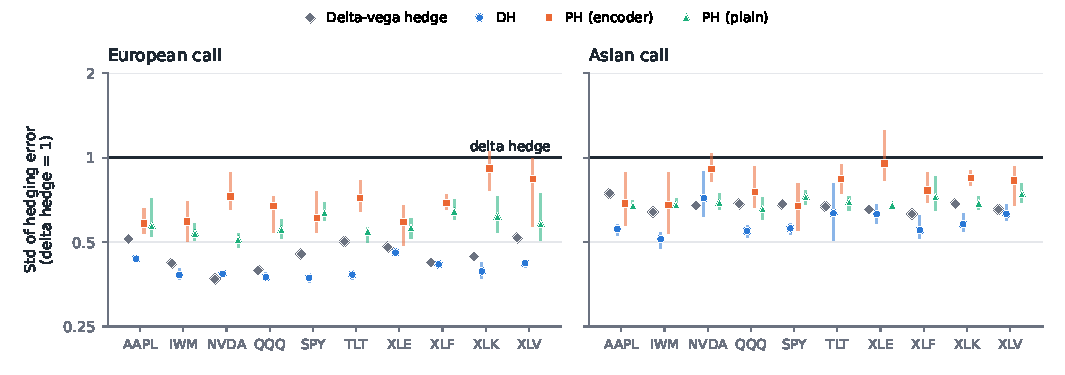
\includegraphics[width=0.92\textwidth]{fig_ticker}
\caption{Standard deviation of the hedging error on the test period by
underlying, relative to the delta hedge, on one logarithmic axis for both
liabilities. Markers are seed means; bars span the five seeds.}
\label{fig:ticker}
\end{figure*}

Table~\ref{tab:main} gives the main result and Table~\ref{tab:contrasts} the
pre-declared contrasts. Three findings stand out.

\emph{Both learned families hedge.} All 300 fits of the three families have
less dispersion than the delta hedge, in every underlying
(Fig.~\ref{fig:ticker}). DH reduces the standard deviation of the hedging
error to 0.40 of the delta hedge's for the European call and 0.61 for the
Asian call; PH to 0.69 and 0.81.

\emph{PH is behind DH.} The difference is significant for both liabilities
and both primary quantities, and PH is behind in all ten underlyings. PH's
standard deviation is 1.7 times DH's for the European call and 1.3 times for
the Asian call. Against the delta--vega hedge, which uses the same two
instruments by formula, DH is ahead in nine of ten underlyings for each
liability, while PH is ahead in none (European) and two (Asian). The plain
layer is better than the encoder layer (0.56 and 0.69 of the delta hedge;
ahead in nine and eight underlyings) but still behind DH.

\emph{Lower dispersion is paid for.} The learned policies and the delta--vega
hedge trade the listed call and pay 0.25--0.39 in costs, against 0.03--0.04
for the delta hedge, so their mean hedging error is lower. The 5\% tail improves
clearly for the European call. For the Asian call no learned policy improves
the tail significantly over the delta hedge.

Results are stable across seeds: the seed-to-seed standard deviation of the
panel figure is at most 4\% (DH), 6\% (PH encoder) and 2\% (PH plain) of
its value. Block lengths of 10 and 40 days change no conclusion.

\subsection{What makes learning work}
\label{sec:ablation}

\begin{table*}[t]
\caption{Variations of the main configuration, test period. ``Std ratio'':
standard deviation of $E$ over the delta hedge's. ``Failed'': fits with more
dispersion than the unhedged position. Other columns in percent of the
initial price. Three seeds unless the denominator shows five.}
\label{tab:arms}
\centering
\footnotesize
\setlength{\tabcolsep}{4pt}
\begin{tabular}{@{}l rrrrr c rrrrr@{}}
\toprule
 & \multicolumn{5}{c}{European call} && \multicolumn{5}{c}{Asian call} \\
\cmidrule{2-6}\cmidrule{8-12}
Variation & Std ratio & $\mathrm{CVaR}_{5\%}(E)$ & Mean $E$ & $\mathrm{CVaR}_{50\%}(O)$ & Failed && Std ratio & $\mathrm{CVaR}_{5\%}(E)$ & Mean $E$ & $\mathrm{CVaR}_{50\%}(O)$ & Failed \\
\midrule
Unhedged & 6.04 & $-$10.75 & $-$0.42 & $-$6.17 & -- && 5.37 & $-$6.38 & $-$0.20 & $-$3.64 & -- \\
Delta hedge & 1.00 & $-$1.48 & +0.07 & $-$3.41 & -- && 1.00 & $-$1.13 & +0.02 & $-$2.10 & -- \\
\multicolumn{12}{@{}l}{\emph{Arm A: variance of $E$, correction to delta}} \\
\quad DH & 0.40 & $-$0.84 & $-$0.30 & $-$3.60 & 0/50 && 0.61 & $-$1.00 & $-$0.32 & $-$2.36 & 0/50 \\
\quad PH (encoder) & 0.69 & $-$1.27 & $-$0.17 & $-$3.55 & 0/50 && 0.81 & $-$1.17 & $-$0.24 & $-$2.30 & 0/50 \\
\quad PH (plain) & 0.56 & $-$1.21 & $-$0.37 & $-$3.74 & 0/50 && 0.69 & $-$1.05 & $-$0.29 & $-$2.34 & 0/50 \\
\multicolumn{12}{@{}l}{\emph{Objective $\mathrm{CVaR}_{10\%}(E)$}} \\
\quad DH & 1.40 & $-$1.67 & +0.39 & $-$3.06 & 0/30 && 1.99 & $-$1.63 & +0.46 & $-$1.72 & 0/30 \\
\quad PH (encoder) & 1.46 & $-$1.94 & +0.45 & $-$3.08 & 0/30 && 1.85 & $-$1.58 & +0.41 & $-$1.81 & 0/30 \\
\multicolumn{12}{@{}l}{\emph{Objective $\mathrm{CVaR}_{50\%}(O)$ (submitted)}} \\
\quad DH & 4.35 & $-$6.59 & +1.42 & $-$3.12 & 5/30 && 6.17 & $-$6.33 & +1.32 & $-$2.05 & 21/30 \\
\quad PH (encoder) & 3.57 & $-$5.02 & +1.11 & $-$3.25 & 0/30 && 4.68 & $-$4.41 & +0.92 & $-$2.16 & 12/30 \\
\multicolumn{12}{@{}l}{\emph{Output is a trade (original semantics)}} \\
\quad DH & 0.49 & $-$0.94 & $-$0.29 & $-$3.62 & 0/30 && 0.66 & $-$1.07 & $-$0.31 & $-$2.34 & 0/30 \\
\quad PH (encoder) & 0.76 & $-$1.44 & $-$0.23 & $-$3.61 & 0/30 && 0.95 & $-$1.27 & $-$0.15 & $-$2.23 & 0/30 \\
\multicolumn{12}{@{}l}{\emph{Original sizes}} \\
\quad DH, width 20 & 0.43 & $-$0.87 & $-$0.29 & $-$3.60 & 0/50 && 0.64 & $-$1.03 & $-$0.30 & $-$2.34 & 0/50 \\
\quad PH (encoder), $K{=}100$ & 0.86 & $-$1.55 & $-$0.12 & $-$3.54 & 0/30 && 0.90 & $-$1.23 & $-$0.17 & $-$2.25 & 0/30 \\
\multicolumn{12}{@{}l}{\emph{One model for all ten tickers}} \\
\quad DH & 0.37 & $-$0.80 & $-$0.33 & $-$3.64 & 0/30 && 0.50 & $-$1.00 & $-$0.45 & $-$2.48 & 0/30 \\
\quad PH (encoder) & 0.47 & $-$1.01 & $-$0.31 & $-$3.65 & 0/30 && 0.60 & $-$1.06 & $-$0.37 & $-$2.40 & 0/30 \\
\quad PH (plain) & 0.55 & $-$1.15 & $-$0.35 & $-$3.71 & 0/30 && 0.66 & $-$1.09 & $-$0.36 & $-$2.42 & 0/30 \\
\multicolumn{12}{@{}l}{\emph{All original settings: trade output, $\mathrm{CVaR}_{50\%}(O)$, original inputs and sizes}} \\
\quad DH, width 20 & 4.29 & $-$7.12 & +0.66 & $-$4.06 & 1/30 && 6.10 & $-$6.76 & +0.76 & $-$2.70 & 23/30 \\
\quad PH (encoder), $K{=}100$ & 4.84 & $-$8.38 & +0.76 & $-$4.05 & 10/30 && 6.12 & $-$6.92 & +0.72 & $-$2.65 & 20/30 \\
\bottomrule
\end{tabular}

\end{table*}

Table~\ref{tab:arms} changes one setting at a time, and then all of them
together.

\emph{The original settings do not produce hedges.} With trade outputs, the
$\mathrm{CVaR}_{50\%}(O)$ objective and the original inputs and sizes (last
block), DH and PH are at parity on the original utility, as in the simulated
study: the difference is $+0.01$ (European) and $+0.05$ (Asian), with
intervals that include zero. But both have four to six times the delta
hedge's dispersion, both score below the delta hedge on that same utility,
and 54 of 120 fits are more dispersed than the unhedged position. Their mean
hedging error is positive: the policies hold directional positions that the
objective cannot tell from a hedge. Changing only the objective to
$\mathrm{CVaR}_{50\%}(O)$ within the main configuration has the same effect.
$\mathrm{CVaR}_{10\%}(E)$ trains without failures but still ends with more
dispersion than the delta hedge.

\emph{Output semantics and size matter less.} With trade outputs and the
variance objective both families still hedge, somewhat worse (DH 0.49 and
0.66, PH 0.76 and 0.95). At the original sizes DH loses little (0.43, 0.64);
PH with $K=100$ loses more (0.86, 0.90). Fewer prototypes generalise better.

\begin{figure*}[t]
\centering
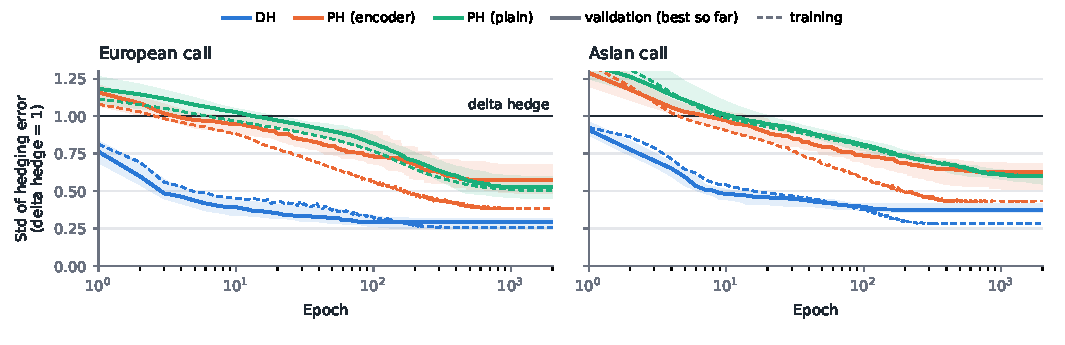
\includegraphics[width=0.92\textwidth]{fig_convergence}
\caption{Training curves of the main configuration (median over 50 fits per
family and liability; band: quartiles of the validation curve). The
untrained policy is the delta hedge.}
\label{fig:conv}
\end{figure*}

\begin{figure}[t]
\centering
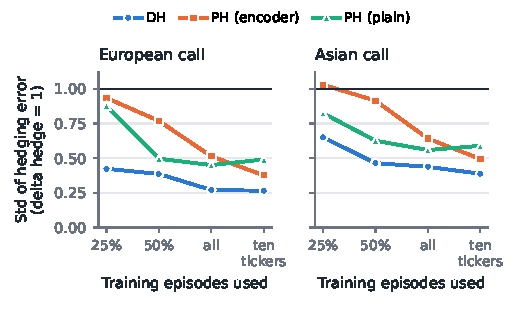
\includegraphics[width=\columnwidth]{fig_data}
\caption{Validation standard deviation of the hedging error against the
amount of training data (SPY, TLT, NVDA; three seeds). ``Ten tickers'': one
model trained on all ten underlyings.}
\label{fig:data}
\end{figure}

\emph{PH needs more data than DH.} Fig.~\ref{fig:conv} shows that every
family converges: no DH fit, 2 of 100 PH (encoder) fits and 13 of 100 PH
(plain) fits reached the epoch limit. The encoder layer overfits: its median
training dispersion falls to 0.38 of the delta hedge's (European) while
validation stays at 0.57; DH's two values are 0.26 and 0.29. The plain layer
shows no such gap. Fig.~\ref{fig:data} varies the training set on validation
data. With a quarter of a ticker's episodes PH (encoder) is no better than
the delta hedge (0.93, 1.03), while DH already reaches 0.42 and 0.65. One
model trained on all ten underlyings helps PH (encoder) most: on the test
period its standard deviation falls from 0.69 to 0.47 of the delta hedge's
(European) and from 0.81 to 0.60 (Asian), against 0.37 and 0.50 for the
pooled DH (Table~\ref{tab:arms}). The pooled PH is thus close to the
per-ticker DH, though still behind the pooled DH. Half of the pooled PH fits
were still improving at their epoch limit, so this is a lower bound on what
pooling gives.

\subsection{Reading a real trade through prototypes}
\label{sec:explain}

\begin{table}[t]
\caption{Explanation diagnostics on all test-period decisions of the main
configuration ($K=10$; means over 100 fits per layer). Distances are
Euclidean in the standardised input space.}
\label{tab:explain}
\centering
\footnotesize
\begin{tabular}{@{}lrr@{}}
\toprule
Diagnostic & Encoder & Plain \\
\midrule
Weight on the heaviest prototype & 0.62 & 0.52 \\
Weight on the three heaviest & 0.92 & 0.84 \\
Effective prototypes per decision & 2.9 & 3.9 \\
Three-prototype reconstruction error & 0.013 & 0.038 \\
\quad relative to the std of the output & 0.04 & 0.09 \\
Heaviest prototype is the nearest state & 28\% & 76\% \\
Median distance rank of the heaviest & 3.7 & 1.0 \\
\bottomrule
\end{tabular}

\end{table}

\begin{table}[t]
\caption{One test-period decision per layer (SPY, European call, seed 0): the
episode with the median hedging error, at the tenth of twenty decisions. Each
prototype is a state from a training episode, shown with that episode's start
date.}
\label{tab:example}
\centering
\scriptsize
\setlength{\tabcolsep}{2.5pt}
\begin{tabular}{@{}lrrrrrr@{}}
\toprule
 & Weight & Spot & Days left & Impl. vol. & \multicolumn{2}{c}{Correction} \\
 & & $S/S_0$ & & & shares & calls \\
\midrule
\multicolumn{7}{@{}l}{\emph{PH (encoder)}: step 10 of the episode starting 2024-07-16} \\
Current state & & 0.960 & 10 & 0.143 & $-$0.036 & $+$0.414 \\
Prototype: 2018-03-09, step 1 & 0.42 & 0.999 & 19 & 0.123 & $-$0.038 & $+$0.520 \\
Prototype: 2015-01-15, step 15 & 0.36 & 1.033 & 5 & 0.167 & $+$0.071 & $+$0.290 \\
Prototype: 2015-10-16, step 7 & 0.11 & 1.016 & 13 & 0.151 & $-$0.136 & $+$0.506 \\
Three-prototype reconstruction & & & & & $-$0.007 & $+$0.425 \\
\addlinespace
\multicolumn{7}{@{}l}{\emph{PH (plain)}: step 10 of the episode starting 2024-05-31} \\
Current state & & 1.029 & 10 & 0.097 & $-$0.195 & $+$0.315 \\
Prototype: 2005-11-15, step 14 & 0.65 & 1.029 & 6 & 0.105 & $-$0.046 & $+$0.096 \\
Prototype: 2014-03-21, step 10 & 0.13 & 1.001 & 10 & 0.118 & $-$0.988 & $+$0.337 \\
Prototype: 2016-10-21, step 3 & 0.10 & 0.999 & 17 & 0.120 & $-$0.006 & $+$0.983 \\
Three-prototype reconstruction & & & & & $-$0.178 & $+$0.229 \\
\addlinespace
\bottomrule
\end{tabular}

\end{table}

An explanation of the form ``this state resembles these past states'' makes
two claims: that the listed prototypes account for the decision, and that
they resemble the current state. Table~\ref{tab:explain} tests both on every
test-period decision. The first claim holds. A decision uses about three to
four prototypes, the three heaviest carry 92\% (encoder) and 84\% (plain) of
the weight, and the output rebuilt from those three differs from the actual
output by 4\% and 9\% of the output's standard deviation.

The second claim depends on the layer. With the released encoder the
heaviest prototype is the nearest prototype in the input space in 28\% of
decisions (3\% to 59\% across fits), where chance is 10\%; its median
distance rank is 3.7 of 10. The encoder is free to place states that look
different next to each other, and it does. With the plain layer the heaviest
prototype is the nearest in 76\% of decisions, and always the nearest in the
layer's own weighted distance. That distance is itself readable: the largest
learned feature weight is on the listed call's moneyness.

Table~\ref{tab:example} shows one decision for each layer, chosen by a fixed
rule. For the encoder layer the two heaviest prototypes lie 19 and 5 days
from the end of their episodes and at different price levels than the
current state. For the plain layer the heaviest prototype has the same
relative price as the current state. In both cases the stated correction is
the weighted average of the prototypes' corrections, which is the sense in
which the policy is transparent.

\section{Limitations}
The liabilities are synthetic and at the money; costs are stylised; daily mid
prices are not executable prices. The rule-based hedges use the listed call's
implied volatility, so they are not model-free references. The ten
underlyings share market shocks, which the bootstrap respects but which
limits the effective sample. The test period had been examined in an earlier
version of the study, so it is held out for these models but not untouched.
Configurations were chosen on three development underlyings and may not be
the best for the other seven. The comparison uses one optimiser and learning
rate for both families; the plain layer in particular often trained up to
the epoch limit. Our conclusions concern PH as released, with fixed
prototypes taken from a DH agent; other ways of placing prototypes are
outside this study.

\section{Reproducibility}
Stage rules, grids and contrasts were written down before the runs they
govern, and the test episodes were opened once with a hashed specification.
Every fit was checked after training: the stored policy is the
validation-best checkpoint, reloading reproduces the saved outcomes, an
independent simulator fed the same positions agrees to $10^{-7}$, and every
prototype is a training-period state. Code, configurations, training curves
and aggregated results will be released; the OptionMetrics and CRSP records
are licensed and cannot be redistributed.

\section*{Acknowledgment}
\pending{AI-assistance disclosure required by IJCNN: to be written by the
authors, naming every tool actually used in the code, analysis and text of
this version.}

\bibliographystyle{IEEEtran}
\bibliography{references}

\end{document}
